\documentclass[12pt]{article}
\usepackage{pgfplots, url, tikz, graphicx}
\usepackage{enumitem} % To customize enumerate
\usepackage{amssymb}
\usepackage{caption}
\usepackage{subcaption}
\usepackage{amsmath}
\usepackage{float}
\usepackage{sagetex}

\usetikzlibrary{arrows.meta, positioning}
\pgfplotsset{compat=1.18}

\title{Math HW Week 7}
\author{Duc Nguyen}
\date{\today}

\begin{document}
\maketitle
\section*{Section 3.4}
\subsection*{\#1}
\begin{align*}
    \begin{cases}
    S' = 0.01ST - 0.2S \\
    T' = 0.05T - 0.01ST
    \end{cases}
\end{align*}
If S' = 0 (no shark), then:
$0 = 0.01ST - 0.2S = S(0.01T - 0.2) => T = 2$
If T' = 0 (no tuna), then:
$0 = 0.05T - 0.01ST = T(0.05 - 0.01S) => S = 5$
\begin{align*}
    \begin{cases}
    S = 5 \\
    T = 2
    \end{cases}
\end{align*}
\subsection*{\#2}
\begin{align*}
    \begin{cases}
    D' = D(3 - M -D) \\
    M' = M(2 - M - 0.5D) \\
    \end{cases}
\end{align*}
To find the M-nullcline, set M' = 0:

$0 = M(2 - M - 0.5D) => 2 - M - 0.5D = 0 => M = 2 - 0.5D$

M-nullcline:
\begin{align*}
    \begin{cases}
    M = 0 \\
    M = 2 - 0.5D
    \end{cases}
\end{align*}

When D = 0, M = 2. The M-nullcline is a line from (0,2) to (4,0).
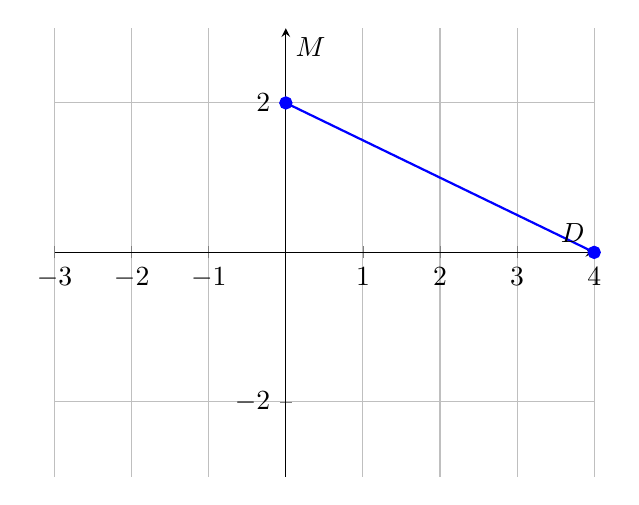
\begin{tikzpicture}
\begin{axis}[
    axis lines = middle, % to place the axes at the center
    xlabel = $D$, % label for x-axis
    ylabel = $M$, % label for y-axis
    grid = both, % shows grid lines
    xmin=-3, xmax=4, % x-axis limits
    ymin=-3, ymax=3  % y-axis limits
]
% Plot the line y = 2x + 1
\addplot[mark=*, blue, thick] coordinates {(0, 2) (4, 0)};
\end{axis}
\end{tikzpicture}
\subsection*{\#3}
Because an equilibrium point is a point where the rate of change is zero, and the nullcline is a line shows the rate of change for each population, when they cross each other, the rate of change is zero for both populations. Hence the equilibrium point is the intersection of the two nullclines.
\subsection*{\#4}
To find the M-nullcline, set M' = 0:
$0 = M(2 - D - M) => 2 - D - M = 0 => M = 2 - D$

M-nullcline:
\begin{align*}
    \begin{cases}
    M = 0 \\
    M = 2 - D
    \end{cases}
\end{align*}
When D = 0, M = 2. The M-nullcline is a line from (0,2) to (2,0) and cut through D-nullcline.

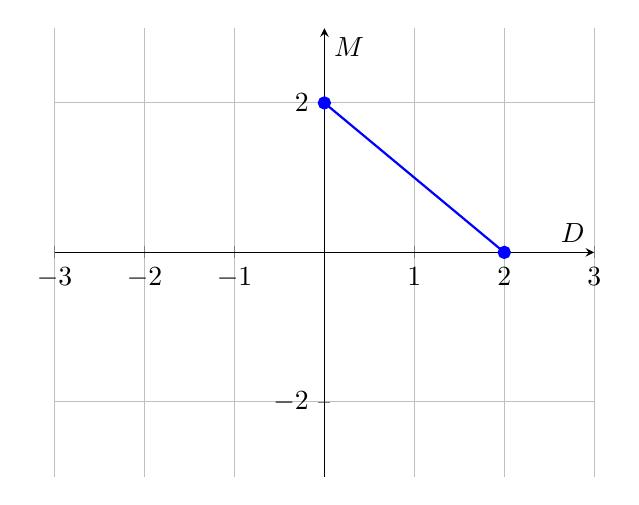
\begin{tikzpicture}
\begin{axis}[
    axis lines = middle, % to place the axes at the center
    xlabel = $D$, % label for x-axis
    ylabel = $M$, % label for y-axis
    grid = both, % shows grid lines
    xmin=-3, xmax=3, % x-axis limits
    ymin=-3, ymax=3  % y-axis limits
]
% Plot the line y = 2x + 1
\addplot[mark=*, blue, thick] coordinates {(0, 2) (2, 0)};
\end{axis}
\end{tikzpicture}

\subsection*{\#5}
with D-nullcline:
\begin{align*}
    \begin{cases}
    D' = 0 \\
    D' = -(1/2)D + 3/2
    \end{cases}
\end{align*}

$0 = -(1/2)D + 3/2 => D = 3$

When D = 3, M = 0. The D-nullcline is a line from (3, 0) and (0, 3/2), cuts through the M-nullcline.

$-(1/2)D + 3/2 = 2 - D => 0 = -(1/2)D + 3/2 - 2 + D => 0 = (1/2)D - 1/2 => D = 1$

$M = 2 - D => 2 - 1 = 1$

The intersection point is (1,1), this is also where the nullcline cross.

Sketching those and we'll have 4 points of intersection:
\begin{align*}
    \begin{cases}
    (0,0) \\
    (0,2) \\
    (1,1) \\
    (3,0)
    \end{cases}
\end{align*}

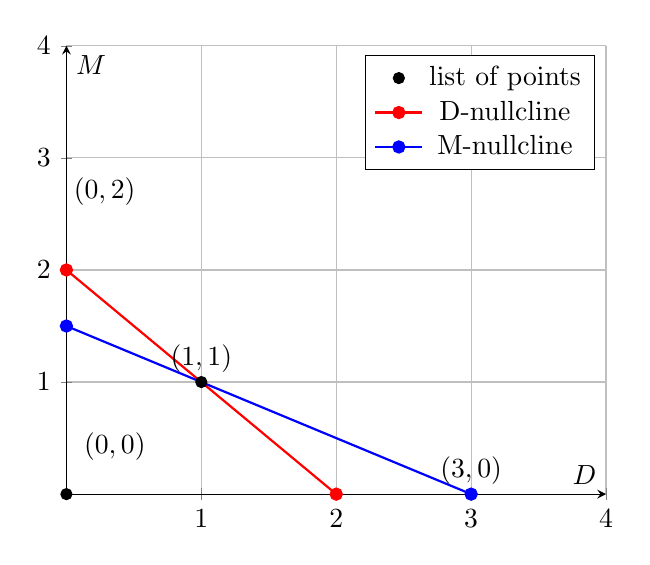
\begin{tikzpicture}
\begin{axis}[
    axis lines = middle, % Position axes in the middle of the graph
    xlabel = $D$, % Label for the x-axis
    ylabel = $M$, % Label for the y-axis
    grid = both, % Add grid lines
    xmin=0, xmax=4, % Set limits for the x-axis
    ymin=0, ymax=4  % Set limits for the y-axis
]
% Plot points on the 2D plane
\addplot[only marks, mark=*] coordinates {(0, 0) (0, 2) (1, 1) (3, 0)};
\addplot[mark=*, red, thick] coordinates {(0, 2) (2, 0)};
\addplot[mark=*, blue, thick] coordinates {(3, 0) (0, 3/2)};

% Label the points
\node at (axis cs:0,0) [xshift=0.1cm, yshift=0.6cm] [anchor=west] {$(0,0)$};
\node at (axis cs:0,2) [xshift=1cm, yshift=1cm] [anchor=east] {$(0,2)$};
\node at (axis cs:1,1) [anchor=south] {$(1,1)$};
\node at (axis cs:3,0) [anchor=south] {$(3,0)$};
\legend{list of points, D-nullcline, M-nullcline}
\end{axis}
\end{tikzpicture}

\subsection*{\#6}
We picked a random point at (1/2, 3/2) to test the direction of the flow. We get those when we plug in the D to the M-nullcline:
\begin{align*}
    0.5 = 2 - M \\
    M = 2 - 0.5 = 1.5 = 3/2
\end{align*}

We then use the D-nullcline to find the direction of the flow:
\begin{align*}
    D' = 3 * 1/2 - 2 * 3/2 * 1/2 - {(1/2)}^2 = -1/4
\end{align*}

The negative value indicates that the flow for the M-nullcline is going towards the left, the change is reversed as it's approaching the equilibrium point.

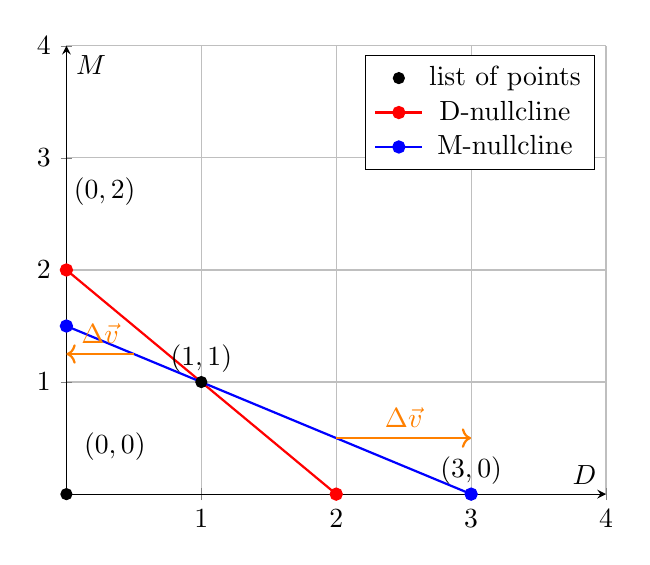
\begin{tikzpicture}
\begin{axis}[
    axis lines = middle, % Position axes in the middle of the graph
    xlabel = $D$, % Label for the x-axis
    ylabel = $M$, % Label for the y-axis
    grid = both, % Add grid lines
    xmin=0, xmax=4, % Set limits for the x-axis
    ymin=0, ymax=4  % Set limits for the y-axis
]
% Plot points on the 2D plane
\addplot[only marks, mark=*] coordinates {(0, 0) (0, 2) (1, 1) (3, 0)};
\addplot[mark=*, red, thick] coordinates {(0, 2) (2, 0)};
\addplot[mark=*, blue, thick] coordinates {(3, 0) (0, 3/2)};
\draw[->, thick, orange] (2,0.5) -- (3,0.5) node[midway, above] {$\Delta \vec{v}$};
\draw[->, thick, orange] (0.5,5/4) -- (0,5/4) node[midway, above] {$\Delta \vec{v}$};

% Label the points
\node at (axis cs:0,0) [xshift=0.1cm, yshift=0.6cm] [anchor=west] {$(0,0)$};
\node at (axis cs:0,2) [xshift=1cm, yshift=1cm] [anchor=east] {$(0,2)$};
\node at (axis cs:1,1) [anchor=south] {$(1,1)$};
\node at (axis cs:3,0) [anchor=south] {$(3,0)$};
\legend{list of points, D-nullcline, M-nullcline}
\end{axis}
\end{tikzpicture}

\subsection*{\#7}
It means that at the intersection of the two nullclines, where the main equilibrium point is, the rate of change for both populations is zero. This means that the populations are stable at that point, if they skewed away too much, the populations will not be able to recover and will die out in both cases.

\subsection*{\#8}
From the model:
\begin{align*}
    \begin{cases}
    N' = 0.05N - 0.01NP \\
    P' = 0.005NP - 0.1P \\
    \end{cases}
\end{align*}

The nullcline for $N'$ will be:
\begin{align*}
    0 = 0.05N - 0.01NP \\
    N(0.05 - 0.01P) = 0 \\
    N = 0 \text{ or } P = 5
\end{align*}

The nullcline for $P'$ will be:
\begin{align*}
    0 = 0.005NP - 0.1P \\
    P(0.005N - 0.1) = 0 \\
    P = 0 \text{ or } N = 20
\end{align*}

The equilibrium point is where both nullclines intersect, which is at (20, 5).

One of the test points is (10, 5) on the N-nullcline, we can find the rate of change for P-nullcline:

\begin{align*}
    P' = 0.005(10)(5) - 0.1(5) = 0.25 - 0.5 = -0.25
\end{align*}

This means that the change before the equilibrium point is negative, and the change after the equilibrium point is positive based on what we know
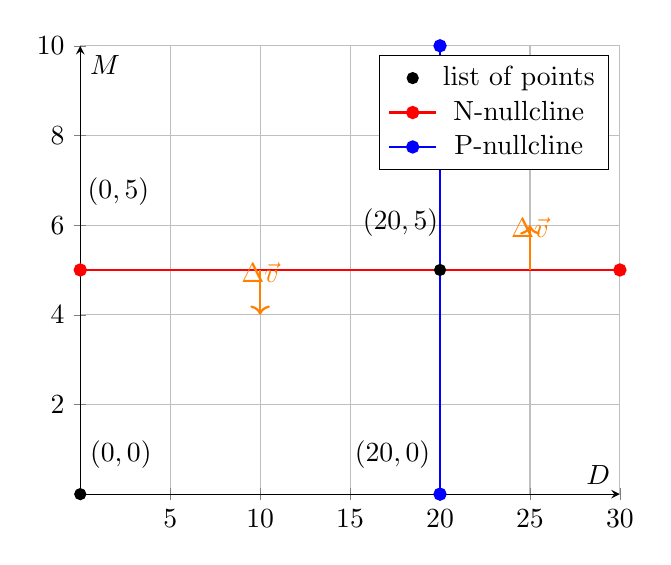
\begin{tikzpicture}
\begin{axis}[
    axis lines = middle, % Position axes in the middle of the graph
    xlabel = $D$, % Label for the x-axis
    ylabel = $M$, % Label for the y-axis
    grid = both, % Add grid lines
    xmin=0, xmax=30, % Set limits for the x-axis
    ymin=0, ymax=10  % Set limits for the y-axis
]
% Plot points on the 2D plane
\addplot[only marks, mark=*] coordinates {(0, 0) (20, 5) (20, 0) (0, 5)};
\addplot[mark=*, red, thick] coordinates {(0, 5) (30, 5)};
\addplot[mark=*, blue, thick] coordinates {(20, 0) (20, 10)};
\draw[->, thick, orange] (10,5) -- (10,4) node[midway, above] {$\Delta \vec{v}$};
\draw[->, thick, orange] (25,5) -- (25,6) node[midway, above] {$\Delta \vec{v}$};

% Label the points
\node at (axis cs:20,5) [xshift=0.1cm, yshift=0.6cm] [anchor=east] {$(20,5)$};
\node at (axis cs:0,5) [xshift=1cm, yshift=1cm] [anchor=east] {$(0,5)$};
\node at (axis cs:20,0) [anchor=east, yshift=0.5cm] {$(20,0)$};
\node at (axis cs:0,0) [anchor=west, yshift=0.5cm] {$(0,0)$};
\legend{list of points, N-nullcline, P-nullcline}
\end{axis}
\end{tikzpicture}

\subsection*{\#9}
The M-nullcline is:
\begin{align*}
    M' = M(r_M - k_M D - c_M M) = 0 \\
    M = 0 \text{ or } D = \frac{r_M - c_M M}{k_M}
\end{align*}

\section*{Further excercises 3.4}
\subsection*{\#1}
\begin{enumerate}[label=\alph*.] 
  \item Because in a predator-prey model, if there's no prey, the predator will die out, and if there's no predator, the prey will grow exponentially. Hence there's no equilibrium point.
  \item Given the model:
\begin{align*}
    \begin{cases}
    N' = rN - aNP \\
    P' = caNP - \delta P
    \end{cases}
\end{align*}
\begin{align*}
    \begin{cases}
    0 = rN - aNP \\
    0 = caNP - \delta P
    \end{cases}
\end{align*}
\begin{align*}
    \begin{cases}
    0 = N(r - aP) \\
    0 = P(caN - \delta)
    \end{cases}
\end{align*}

\begin{align*}
    \begin{cases}
    N = 0 \quad \text{or} \quad P = r / a \\
    P = 0 \quad \text{or} \quad N = \frac{\delta}{ca}
    \end{cases}
\end{align*}
\end{enumerate}
The equilibrium point after solving the system is ($\frac{\delta}{ca}, \frac{r}{a}$).

\subsection*{\#2}
Given the equation:
\begin{align*}
    \begin{cases}
    N' = rN(1 - N / 5000) - 0.01NP \\
    P' = 0.001NP - 0.001P
    \end{cases}
\end{align*}

We can find the equilibrium point by setting $N' = 0$ and $P' = 0$:
\begin{align*}
    \begin{cases}
    0 = (0.1)N(1 - N / 5000) - 0.01NP \\
    0 = 0.001NP - 0.001P
    \end{cases}
\end{align*}

We can simplify the second equation:
\begin{align*}
    0 = P(0.001N - 0.001) \\
    P = 0 \quad \text{or} \quad N = 1
\end{align*}
which gives 2 points: $N = 1$ and $P = 0$, leads to 2 different cases.

If $P = 0$, plugging it into the first equation will gives:
\begin{align*}
    0 = rN(1 - N / 5000) \\
    N = 0 \quad \text{or} \quad N = 5000
\end{align*}

This means that there's 2 equilibrium points: (0,0) and (5000,0).

If $N = 1$, plugging it into the first equation will gives:
\begin{align*}
    0 = 0.1(1)(1 - 1 / 5000) - 0.01(1)P \\
    0 = 0.1(1 - 1 / 5000) - 0.01P \\
    P = 10(1 - 1 / 5000) \\
    P \approx 9.998
\end{align*}

We have an another equilibrium: (1, 9.998).
In total, we have 3 equilibrium points:
\begin{align*}
    \begin{cases}
    (0, 0) \\
    (5000, 0) \\
    (1, 9.998)
    \end{cases}
\end{align*}

\subsection*{\#3}
\begin{figure}[htbp]
    \centering
    \includegraphics[width=0.8\textwidth]{Hw7.png}
\end{figure}

For each equilibrium, at (0,0), where both population extinct, the flow is unstable, at (5000,0), where the prey population is stable but no predator, the flow converge to an unstable, and at (1,9.998), where both population are converge and stable, the flow is stable as well, which I assume that it has some shape of a saddle point where it converge to (1,9.998).

Compared to Lotka-Volterra, it has a neutral cycles, 2 equilibrium, unlimited prey growth. This system instead has a logistic term in prey growth and predator decay.

\subsection*{\#6}
\begin{enumerate}[label=\alph*.] 
    \item Given the model:
\begin{align*}
    \begin{cases}
    D' = 0.3D - 0.02D^2 - 0.05DM \\
    M' = 0.2M - 0.04M^2 - 0.02DM
    \end{cases}
\end{align*}
\begin{align*}
    \begin{cases}
    0 = 0.3D - 0.02D^2 - 0.05DM \\
    0 = 0.2M - 0.04M^2 - 0.02DM
    \end{cases}
\end{align*}
\begin{align*}
    \begin{cases}
    0 = D(0.3 - 0.02D - 0.05M) \\
    0 = M(0.2 - 0.04M - 0.02D)
    \end{cases}
\end{align*}
\begin{align*}
    \begin{cases}
    D = 0 \text{or} M = (0.3 - 0.02D) / 0.05 \\
    M = 0 \text{or} D = 2M - 10
    \end{cases}
\end{align*}

\begin{figure}[htbp]
    \centering
    \includegraphics[width=0.8\textwidth]{hw7_2.png}
\end{figure}
\item We can find the equilibrium point for both
\begin{align*}
    D(0.3-0.02D-0.05M)=0 \\
    D = 0 => M(0.2-0.04M)=0 => M=0 \text{or} M=5 => (0,0),(0,5) \\
\end{align*}
For the other nullcline:
\begin{align*}
    M(0.2-0.04M-0.02D)=0 \\
    M = 0 => D(0.3-0.02D)=0 => D=0 \text{or} D=15 => (15,0)
\end{align*}
The intersection of the two nullclines, which gives the stable equilibrium point, is $(D,M) = (6,1.2)$ if you use a numerical method to solve the system since the algebraic way doesn't work.
\item \begin{figure}[htbp]
    \centering
    \includegraphics[width=0.8\textwidth]{hw7_3.png}
\end{figure}
\item At (0, 0), both populations extinct, hence unstable. At (15, 0), only deer survive but no moose, the deer population will grow exponentially, hence unstable. At (0, 5), only moose survive, hence it's unstable as well, in decreasing terms. At (6,1.2), both population survive, means that it's stable
\item With the following answer, we can see that for both deer and moose to survive, the moose population must be at least 1.2 and the deer population must be at least 6. It's also where the main equilibrium point is.
\end{enumerate}

\end{document}